% Created 2013-03-12 Tue 10:30
\documentclass[11pt]{article}
\usepackage[utf8]{inputenc}
\usepackage[T1]{fontenc}
\usepackage{fixltx2e}
\usepackage{graphicx}
\usepackage{longtable}
\usepackage{float}
\usepackage{wrapfig}
\usepackage{soul}
\usepackage{textcomp}
\usepackage{marvosym}
\usepackage{wasysym}
\usepackage{latexsym}
\usepackage{amssymb}
\usepackage{hyperref}
\tolerance=1000
% examformat.tex
% set up page formatting for exams/quizzes

% page margins
\usepackage[letterpaper]{geometry}
\geometry{verbose, tmargin = 1in, bmargin = 1in, lmargin = 1in, rmargin = 1in}

% format headings for questions/answers
\usepackage{titlesec}
\titleformat{\section}[runin]{\normalfont}{\bfseries\arabic{section}.}{.5em}{}[\quad]
\titleformat{\subsection}[block]{\normalfont}{\bfseries\alph{subsection})}{.5em}{}[\quad]
\titleformat{\subsubsection}[block]{\normalfont}{}{}{}[\quad]

% typeset student entered R code
\newenvironment{studinpt}
  {\begin{minipage}{\textwidth}\ttfamily}
  {\end{minipage}}

% extra math commands
\newcommand{\E}{\mathrm{I\! E}}
\renewcommand{\P}{\mathrm{I\! P}}

% extra space between last line of text and footnote rule
\skip\footins 20pt plus4pt minus4pt

\date{\vspace{-0.5in}Sample Quiz Template}
\title{\vspace{-0.5in}\large STAT 1234 | SOME STATISTICS CLASS | SPRING 2013 | KERNS}
\hypersetup{
  pdfkeywords={},
  pdfsubject={},
  pdfcreator={Generated by Org mode 8.0-pre in Emacs 24.3.50.1.}}
\begin{document}

\maketitle
\begin{flushright}
Name: \underbar{\makebox[2in]{}}
\par
\end{flushright}
\vspace{0.1in}

\noindent \textbf{Directions:\footnote{more questions on the back.}} SHOW ALL WORK. You may use \texttt{R} for
computations, but no other software (and in particular, not the
Internet). If you use \texttt{R} to calculate something, then hand-write the
\texttt{R} code that you typed, together with the numerical answer.

\section[The following table categorizes a group of people based on the flavor of Kool-Aid they drink and whether or not they like President Barack Obama.]{The following table categorizes a group of people based on the flavor of Kool-Aid they drink and whether or not they like President Barack Obama.}
\label{sec-1}

\begin{center}
\begin{tabular}{lrrrr}
 & grape & orange & cherry & Total\\
\hline
likes Obama & 92 & 93 & 29 & 214\\
doesn't like Obama & 84 & 64 & 51 & 199\\
Total & 176 & 157 & 80 & 413\\
\end{tabular}
\end{center}

Our experiment will be to select one (1) person from the table out
of the 413 people, at random.

\subsection[What is the probability that the selected person likes cherry Kool-Aid?]{What is the probability that the selected person likes cherry Kool-Aid?}
\label{sec-1-1}
\subsubsection[]{}
\label{sec-1-1-1}
\begin{quote}
Since all outcomes are equally likely, the marginal probability that
the person likes cherry Kool-Aid is just the number
of people who like cherry Kool-Aid divided by the
total number of people in the study.  In other words,

\[
\P( \mbox{cherry}) = \frac{\mbox{\#(cherry)}}{\mbox{Total \# of people}} = \frac{80}{413}\approx 0.194.
\]

\end{quote}
\subsection[What is the probability that the selected person doesn't like Obama?]{What is the probability that the selected person doesn't like Obama?}
\label{sec-1-2}
\subsubsection[]{}
\label{sec-1-2-1}
\begin{quote}
This problem is just like the last problem, but we are thinking about rows instead of columns. In particular,

\[
\P( \mbox{doesn't like Obama}) = \frac{\mbox{\#(doesn't like Obama)}}{\mbox{Total \# of people}} = \frac{199}{413}\approx 0.482.
\]

\end{quote}
\subsection[What is the conditional probability that the person likes grape Kool-Aid, given that the person doesn't like Obama?]{What is the conditional probability that the person likes grape Kool-Aid, given that the person doesn't like Obama?}
\label{sec-1-3}
\subsubsection[]{}
\label{sec-1-3-1}
\begin{quote}
To calculate the conditional probability we restrict attention to the row that contains a person who doesn't like Obama, and out of those total people calculate the proportion of those who like grape Kool-Aid, that is,

\[
\P( \mbox{ grape } \vert \mbox{ doesn't like Obama } ) = \frac{\P( \mbox{grape and doesn't like Obama} )}{\P(\mbox{ doesn't like Obama} ) } = \frac{84}{199} \approx 0.422.
\]

\end{quote}
\section[We would like to feed baby ``Aidan''. At the dinner table, we get a spoon of food and make an airplane \emph{swoop} as we move the spoon toward his mouth.]{We would like to feed baby ``Aidan''. At the dinner table, we get a spoon of food and make an airplane \emph{swoop} as we move the spoon toward his mouth.}
\label{sec-2}

Calling the event \( E = \left\{ \mbox{take a bite}\right\} \) a
``success'', it has been determined by experimentation that on any
given airplane swoop, the probability of success is \(p \approx\)
0.39. Suppose that Aidan is in the high chair. Let \(Y\) denote the
number of failed swoops (\(E^{c}=\left\{ \mbox{no bite}\right\}\))
before the first 6 successful bites.

\subsection[If the successive swoops were to constitute independent Bernoulli trials, what would be the distribution of \(Y\)? You should write the family name of the distribution and numerical value(s) of a(ny) parameter(s).]{If the successive swoops were to constitute independent Bernoulli trials, what would be the distribution of \(Y\)? You should write the family name of the distribution and numerical value(s) of a(ny) parameter(s).}
\label{sec-2-1}

\subsubsection[]{}
\label{sec-2-1-1}
\begin{quote}
The distribution of \(Y\) is \emph{negative binomial} with \texttt{size} equal to
6 and \texttt{prob} equal to 0.39.  The following \texttt{R} code will
suffice to communicate this to the computer.

\begin{verbatim}
library(distr)
Y <- Nbinom(size = 6, prob = 0.39)
\end{verbatim}

\end{quote}
\subsection[Find the mean and variance of \(Y\), denoted \(\E Y\) and \(\mathrm{Var}(Y)\), by any method you like.]{Find the mean and variance of \(Y\), denoted \(\E Y\) and \(\mathrm{Var}(Y)\), by any method you like.}
\label{sec-2-2}
\subsubsection[]{}
\label{sec-2-2-1}
\begin{quote}
The mean of the \texttt{Nbinom(size = r, prob = p)} distribution is \(r(1 - p)/p\) and the variance is \(r(1 - p)/p^2\).  You can either calculate that by hand or you can use the computer via the \texttt{distrEx} package:

\begin{verbatim}
library(distrEx)
E(Y)
var(Y)
\end{verbatim}

\begin{verbatim}
[1] "\\P( \\mbox{doesn't like Obama}) = \\frac{\\mbox{\\#(doesn't like Obama)}}{\\mbox{Total \\# of people}} = \\frac{199}{413}\\approx 0.482"
[1] "grape"
[1] "doesn't like Obama"
[1] "doesn't like Obama"
[1] "grape"
[1] "\\P( \\mbox{ grape } \\vert \\mbox{ doesn't like Obama } ) = \\frac{\\P( \\mbox{grape and doesn't like Obama} )}{\\P(\\mbox{ doesn't like Obama} ) } = \\frac{84}{199} \\approx 0.422."
[1] "\\P( \\mbox{ grape } \\vert \\mbox{ doesn't like Obama } ) = \\frac{\\P( \\mbox{grape and doesn't like Obama} )}{\\P(\\mbox{ doesn't like Obama} ) } = \\frac{84}{199} \\approx 0.422."
[1] 0.39
[1] 6
[1] 6
[1] 0.39
[1] "Y <- Nbinom(size = 6, prob = 0.39)"
[1] "Y <- Nbinom(size = 6, prob = 0.39)"
[1] 9.384615
[1] 24.06312
\end{verbatim}

\end{quote}
\subsection[Sketch the probability mass function of \(Y\) (roughly). It does not have to be exact, but it should have the right support, be centered in the right place, and have the correct basic spread and shape.]{Sketch the probability mass function of \(Y\) (roughly). It does not have to be exact, but it should have the right support, be centered in the right place, and have the correct basic spread and shape.}
\label{sec-2-3}

\subsubsection[]{}
\label{sec-2-3-1}
\begin{quote}
See Figure \ref{fig-pmf}; your sketch should look something like that.  The \texttt{R} code you can use to make the figure is:

\label{pmf}
\begin{verbatim}
plot(Y, to.draw.arg = "d")
\end{verbatim}

\begin{figure}[htb]
\centering
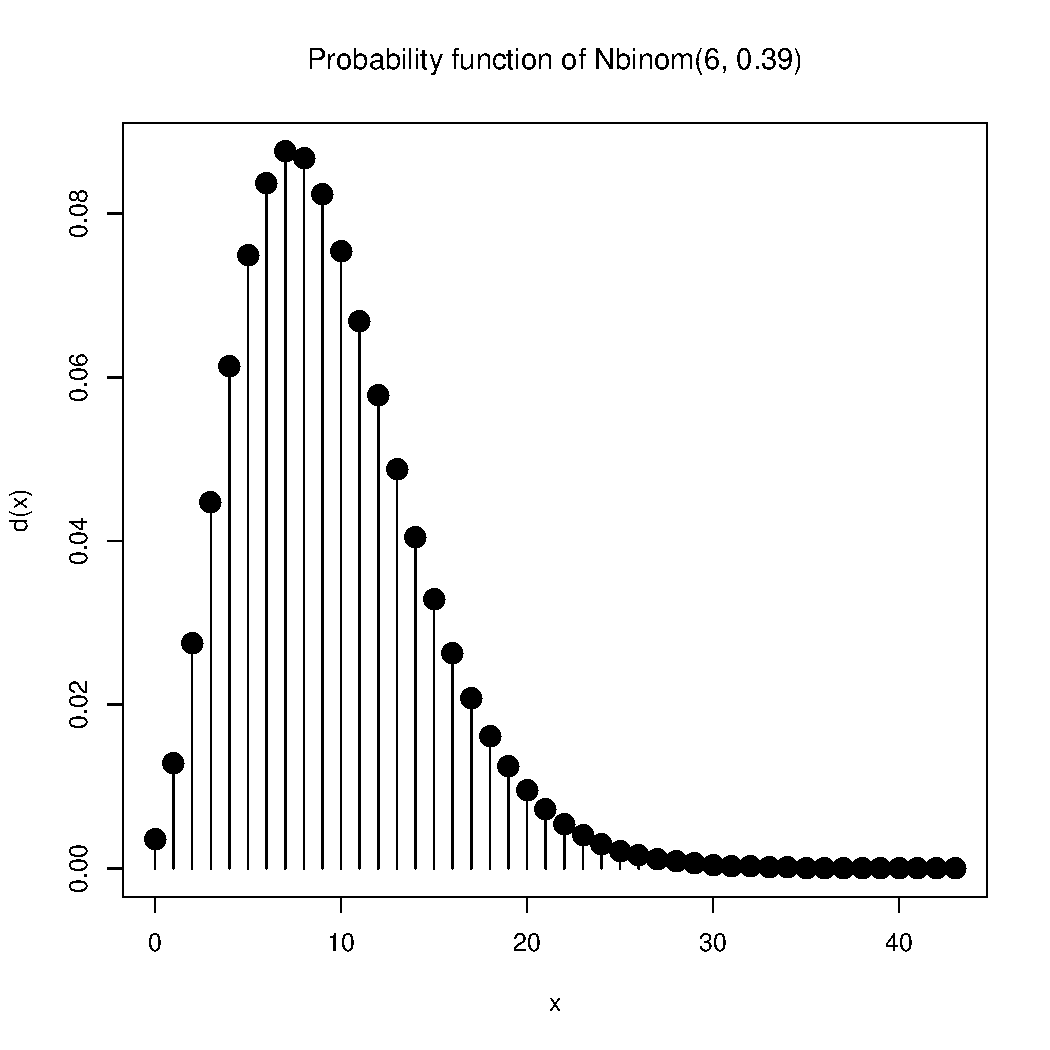
\includegraphics[width=6cm]{plotpmf.pdf}
\caption{\label{fig-pmf}Plot of the probability mass function}
\end{figure}

\end{quote}
% Generated by Org mode 8.0-pre in Emacs 24.3.50.1.
\end{document}